\documentclass[journal, 10pt]{IEEEtran}
\usepackage[utf8]{inputenc}
\usepackage[spanish,es-noshorthands]{babel}
\usepackage{amsfonts}
\usepackage{amsmath}
\usepackage{graphicx}
\usepackage{url}
\def\IEEEkeywordsname{Palabras Claves}

\makeatletter
\long\def\@makecaption#1#2{\ifx\@captype\@IEEEtablestring%
\footnotesize\begin{center}{\normalfont\footnotesize #1}\\
{\normalfont\footnotesize\scshape #2}\end{center}%
\@IEEEtablecaptionsepspace
\else
\@IEEEfigurecaptionsepspace
\setbox\@tempboxa\hbox{\normalfont\footnotesize {#1.}~~ #2}%
\ifdim \wd\@tempboxa >\hsize%
\setbox\@tempboxa\hbox{\normalfont\footnotesize {#1.}~~ }%
\parbox[t]{\hsize}{\normalfont\footnotesize \noindent\unhbox\@tempboxa#2}%
\else
\hbox to\hsize{\normalfont\footnotesize\hfil\box\@tempboxa\hfil}\fi\fi}
\makeatother

\newtheorem{example}{Ejemplo}

\begin{document}
\title{\textit{Knight's Tour:  El problema del Caballo}}
\author{Ignacio Figueroa Ram\'irez \\Sebasti\'an Herrera Corrales\\ Felipe Samur Sansur\\ Universidad T\'ecnica Federico Santa Mar\'ia \\ Avenida Vicu\~na Mackenna 3939,San Joaqu\'in, Santiago, Chile \\
\{ignacio.figueroara, sebastian.herrerac, jorge.samur\}@sansano.usm.cl}
\maketitle

\begin{abstract}
\textbf{El protagonista de este art\'iculo es el \textit{Knight's Tour Problem}, un antiguo problema matemático que hasta el día de hoy sigue siendo de interés, debido a que gira en torno al caballo del ajedrez, la pieza que sin duda tiene el movimiento más curioso del set, y a la gran cantidad de soluciones que se le han encontrado. En el artículo se verá un pequeño repaso histórico del problema y conceptos propios de éste, luego se verá en profundidad en qué consiste el problema y como puede ser abordado y solucionado de distintas maneras, y para finalizar se expondrá sobre instancias notables y problemas relacionados. }
\end{abstract}

\begin{IEEEkeywords}
Knight's Tour Problem, Camino Hamiltoniano, Regla de Warnsdorff, Método Divide y Vencerás.
\end{IEEEkeywords}

\section{Introducci\'on}
El \textit{Knight's Tour Problem} (KTP), o Problema del Caballo, tiene como objetivo encontrar una ruta o camino en un tablero de ajedrez tal que el caballo visite todas las celdas del tablero una sola vez.
El primer \textit{problema del caballo} data del siglo séptimo en un manuscrito árabe titulado \textit{La delicia de los inteligentes, una descripción del ajedrez} y contiene dos soluciones \cite{Murray:1913}. Sin embargo, no fue hasta 1766 que el problema fue analizado por primera vez en un artículo matem\'atico \cite{Euler:1759} por el conocido Leonhard Euler, art\'iculo que sentó las bases para ensayos futuros. El concepto de este problema puede ser aplicado en procesamiento de imágenes, dado que el tablero de ajedrez puede emular una matriz de píxeles \cite{Xiaoyong:2017}.\\
En las siguientes secciones se profundizará m\'as acerca de este problema. En la secci\'on $II$ se profundizar\'a acerca de los movimientos que puede realizar el caballo, se presentar\'a el problema y se explicar\'a mas detalladamente con un ejemplo. La secci\'on $III$ se enfocará en dar contexto acerca de algunas soluciones del problema, como también de problemas previos a éste. Finalmente se presentar\'an conclusiones y expectativas para el desarrollo de este problema es futuros informes.

%Fundamentación histórica del problema. No olvide citar sus fuentes . Desarrolle en prosa respondiendo las siguientes preguntas: ¿Sobre qué necesidad fue construido el problema? ¿Cuál es su origen? ¿Qué busca solucionar? ¿Por qué se hace interesante resolver el problema? ¿Cómo se aplica en la vida real? Además, no olvide mencionar que abarcará en ésta entrega y cómo estará estructurado el artículo a partir de la siguiente sección (20 pts.).

\section{El Problema}
De los seis trebejos del juego de ajedrez, este art\'iculo se concentrará en uno de éstos y en un problema preciso asociado a éste. El caballo tiene un movimiento inusual entre las piezas de ajedrez, se puede desplazar dos casillas horizontalmente y una casilla verticalmente o dos casillas en posición vertical y una horizontal. Con lo cual, el movimiento completo se parece a la letra "$\mathcal{L}$"  \cite{Uehara:2019}.

\begin{figure}[h]

\centering
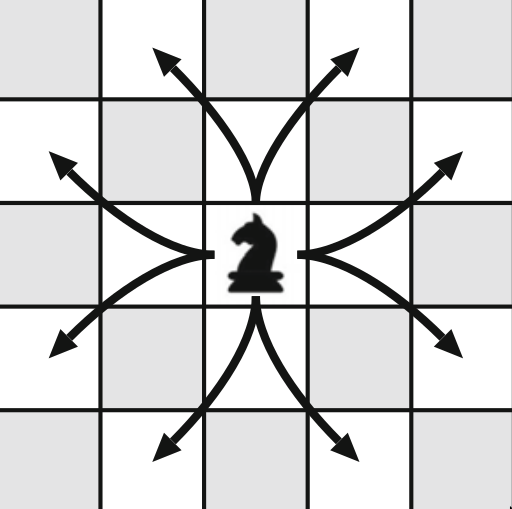
\includegraphics[width=0.15\textwidth]{figures/k_moves.png}
\caption{Movimientos del caballo en un tablero de ajedrez.}
\label{fig:moves}

\end{figure}

El problema del caballo consiste en encontrar una ruta para el caballo en un tablero de ajedrez de tamaño $n \times m$, de modo que éste visite cada casilla una sola vez. La soluci\'on de este problema se representa como una matriz numerada que indica el orden que sigui\'o el caballo para completar el camino \cite{Kopec:2016}.

\begin{example}
	Una de las soluciones que encontró Euler y que publicó en \cite{Euler:1759} es especialmente interesante ya que trabaja con las simetr\'ias del tablero. Euler primero realiza un recorrido por la mitad inferior del tablero, comenzando en el cuadrado $1$ y terminando en el cuadrado $32$. Luego repite exactamente este mismo recorrido, de manera sim\'etrica, para la parte superior mitad del tablero, comenzando en el cuadrado $33$ y terminando en el cuadrado $64$. El ejemplo se ve a detalle en la \textit{Figura \ref{fig:euler}} 
\end{example}

\begin{figure}[h]

\centering
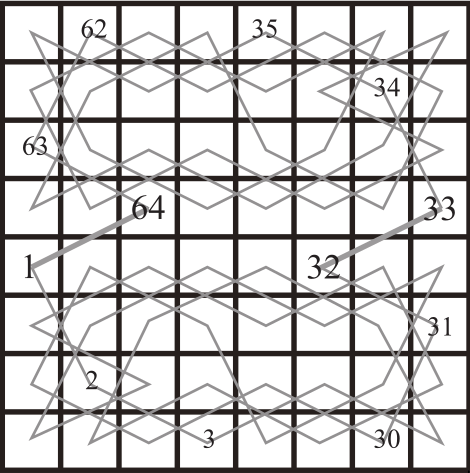
\includegraphics[width=0.15\textwidth]{figures/EulerKT.png}
\caption{Soluci\'on propuesta por Euler en 1759.}
\label{fig:euler}

\end{figure}
%En que consiste el problema, sobre que necesidad fue construido y comentarios generales. Preguntas claves: ?`En que consiste mi problema??`Cuales son sus origines??`Que quiero solucionar? (10 ptos) .\\
\section{Estado del arte}
Hay soluciones que tienen todo tipo de enfoques; pueden ser para tableros de una dimensión fija, otras soluciones pueden servir para cualquier dimensión otorgada al tablero, otros solo para casos pequeños, otros dentro de un rango de dimensiones, etc. A continuación se muestran algunos algoritmos que se han diseñados para resolver el problema a lo largo de la existencia del enigma matemático.

La primera solución al problema son las demostraciones desarrolladas por Parberry \cite{Parberry:1997}, quien propone un acercamiento de tipo “dividir y conquistar”. En pocas palabras, Parberry propone separar el tablero en subsecciones de tamaño similar y completar el tour en cada una de estas subsecciones antes de pasar a la siguiente. La propuesta considera distintas demostraciones para distintos tipos de tablero, sin embargo todas se basan en el mismo principio. Este método posee varias ventajas, como su simpleza, ya que las técnicas son fáciles de entender y demostrar \cite{Parberry:1997}, y también su eficiencia, pues poseen complejidad $\mathcal{O}(n^2)$, lo que implica un tiempo proporcional a la superficie del tablero y por lo tanto lineal en cuanto al área (para un tablero no cuadrado la complejidad sería $\mathcal{O}(n\times m) $ con \textit{n,m} las dimensiones del tablero). Por el contrario, la mayor desventaja del método es que no existe una regla general, es decir a pesar que todos los teoremas comparten la misma base, la elección va a depender de la configuración $m\times n$ del tablero.

Otra técnica es "El Algoritmo de Warnsdorff" (para el problema del caballo), el cual funciona para tableros con dimensión mínima de $5\times 5$ y consiste en visitar las casillas menos asequibles lo más pronto posible con la finalidad de evitar posibles caminos sin salida y/o arrinconados en un futuro. La Heurística de Warnsdorff \cite{Squirrel:1996}, dice:
\begin{quote}
	Habiendo iniciado el camino de una casilla arbitraria: sea la $(n+1)$-ésima casilla del camino (siendo n la cantidad actual de casillas recorridas), entonces esta casilla:
	\begin{enumerate}
		\item Está al alcance de la n-ésima casilla
		\item Aún no ha sido visitada previamente.
		\item Es la casilla desde la cual menos movimientos es posible hacer de todas las casillas alcanzables no visitadas de la n-ésima casilla.
\end{enumerate}
\end{quote}

\begin{figure}[h]
\centering
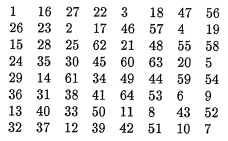
\includegraphics[width=0.2\textwidth]{figures/warnsdorff.png}
\caption{Soluci\'on hecha siguiendo la Heurística de Warnsdorff}
\label{fig:warnsdorff}
\end{figure}
Sin embargo, pueden se pueden presentar situaciones en que 2 casillas cumplan con las mismas condiciones. Aquí es donde nace la imperfección del algoritmo, pues si bien existen criterios de desempate que han sido creados después de numerosos estudios del algoritmo y tienden a permitir elegir el camino correcto, no son metodologías del todo exactas y pueden aún así originarse dilemas difíciles de resolver a la hora de elegir un camino, y si se toma una mala decisión el camino podría no terminarse. Además, la Heurística de Warnsdoff no es confiable por si sola para tableros de dimensiones muy grandes (p.e. $n \geq 200)$, pues estos enfrentamientos de desempate se hacen más recurrentes. Aún así, la Heurística de Warnsdorff es bastante efectiva para los rangos sugeridos y una buena opción gracias a su patrón intuitivo y simpleza.   

Siguiendo con algunas instancias del problema que son interesantes de resolver, dadas las características específicas del problema los casos de estudio siempre se relacionan con la forma del tablero $m \times n$. De éstas, quizás la más popular es la del tablero de ajedrez $8 \times 8$, la cual fue resuelta por Euler \cite{Euler:1759} hace siglos atrás. Parberry \cite{Parberry:1997} describe otros casos más específicos, tales como el tablero $n \times n$, $n \ge 5 \wedge n=\text{impar}$, en el cual existen tours cerrados que pasan por todos los espacios a excepción de una de las esquinas; tours para tableros de tipo $n \times (n+1), n \ge 6$ y algunas propiedades interesantes relacionadas con la simetría de tours para tableros $n \times n, n \ge 10, n$ divisible por $2$ pero no por $4$. Destacar que para cualquier caso, el tablero $n \times n$ mínimo para trabajar es el de $5\times 5$, ya que de considerar $n$ inferior a $5$ existirían espacios inalcanzables.

En cuanto a aportes del problema, no se han encontrado otros problemas que se vean beneficiados de su aplicación, existen casos particulares como una famosa partida de un torneo de ajedrez en la que uno de los participantes realizó 13 movimientos consecutivos que parecían seguir un Knight's Tour\cite{Shabazz:2010}.

Por útlimo, un problema que benefició el entendimiento del problema del caballo es el de encontrar un camino hamiltoniano. Un camino de hamiltoniano es un camino que visita cada nodo de un grafo exactamente una vez, y de hecho un camino del caballo (para el problema) corresponde a un camino hamiltoniano en un grafo cuyos nodos representan las casillas  del tablero, y dos nodos est\'an conectados si un caballo puede moverse entre las casillas seg\'un las reglas del ajedrez \cite{Rosen/2002}. Los variados algoritmos que sirven para resolver el problema de encontrar un camino hamiltoniano en un grafo simplifican el desarrollo del problema del caballo. Sin embargo, se presentaron dos enfoques más apropiados para el caso.

% Desarrollo científico del problema. Investigar y recopilar información de como el problema ha sido abordado y/o solucionado. Explique las ventajas y defectos de los distintos enfoques aplicados (si es necesario se recomienda generar una tabla para resumir las técnicas y su información). \textit{Sea crítico en los defectos, y no endiose en los aciertos}. Además, comente sobre instancias (casos específicos) del problema que son reconocidos en la comunidad científica y los desafíos de solucionar éstos. No olvide mencionar sobre problemas similares, afines o análogos. Infiera como resoluciones de problemas similares pueden aportan grandes ideas para el desarrollo de su problema, pero sin ser explicito (\textit{hint: un mago no revela sus trucos de magia}). Desarrolle en prosa respondiendo las siguiente interrogantes: ¿Qué técnicas se han implementado? ¿Cuáles son sus ventajas y desventajas? ¿Qué instancias son interesantes de resolver? ¿Que otros problema han sido beneficiados de éste? ¿Que otros problemas han beneficiado a éste?. Considere que \textbf{debe} incluir referencias por cada técnica o solución analizada y mencionada (30 pts.).

\section{Conclusiones y Perspectivas}
El Knight’s Tour es un problema que ha sido ampliamente desarrollado tanto por matemáticos como informáticos, ya que al ser un caso particular de un problema de Hamilton su desarrollo resulta de gran interés para aportar al entendimiento general de esta categoría de problemas. Lo relevante del problema es cómo el mismo procedimiento (el movimiento del caballo) se puede aplicar a distintas configuraciones según el problema específico (las características del tablero), siendo necesario para mejorar su resolución la búsqueda de un método general y eficiente que se pueda aplicar a cualquier configuración.

Lo que se hará a futuro es buscar la formulación del enunciado en el contexto de un problema de optimización, así como la investigación correspondiente para poder lograr este objetivo de manera formal y sin errores como debe ser. También, al ser éste un problema común en el área de informática, se podría trabajar en el futuro con programas enfocados a resolver distintos Knight’s tours, con el fin de poder lograr una mejor comprensión del problema.

%Desarrollo de los aportes de la entrega, resultados y de los futuros pasos a seguir tanto como para las próximas entregas como para desarrollos fuera del curso. El orden es siempre, aportes y en párrafo aparte los trabajos futuros y/o perspectivas. Desarrolle en prosa respondiendo lo siguiente: ¿Cuál es el aporte del problema? ¿Qué es relevante del problema y como se puede seguir mejorando su resolución? ¿Qué se hará a futuro? ¿Qué se podría hacer a futuro? (10 pts.).

\section{Referencias}
\bibliography{bibliografia}
\bibliographystyle{ieeetr}
\end{document}
